\documentclass{article}

% -----------------------------------------------------------------------------
% English Comments Added for Clarity
% This document is a LaTeX file for a homework assignment. The original text is
% in Persian. The comments below are added to explain the structure and packages
% used in the document.
% -----------------------------------------------------------------------------

% --- Package Loading ---
% The following section loads the necessary LaTeX packages for this document.

% The 'neurips' style file is used for formatting, likely from a template for the
% Neural Information Processing Systems (NeurIPS) conference. The [final] option
% indicates that this is the camera-ready version.
\usepackage[final]{neurips}

% 'multicol' allows for text to be set in multiple columns.
\usepackage{multicol}

% 'float' provides improved control over floating objects like figures and tables.
\usepackage{float}

% 'caption' is used for customizing the captions of figures and tables.
\usepackage[center]{caption}

% 'inputenc' with the [utf8] option allows for UTF-8 encoded text to be used directly.
\usepackage[utf8]{inputenc}

% 'fontenc' with the [T1] option specifies the font encoding.
\usepackage[T1]{fontenc}

% 'hyperref' creates hyperlinks within the document (e.g., for references and URLs).
\usepackage{hyperref}

% 'url' provides a simple way to format URLs.
\usepackage{url}

% 'booktabs' is used for creating professional-quality tables.
\usepackage{booktabs}

% 'amsfonts' provides access to blackboard bold math symbols.
\usepackage{amsfonts}

% 'nicefrac' allows for the typesetting of compact fractions.
\usepackage{nicefrac}

% 'microtype' improves the typographic quality of the document.
\usepackage{microtype}

% 'graphicx' is used for including images in the document.
\usepackage{graphicx}

% 'amsmath' provides a wide range of environments for typesetting mathematical formulas.
\usepackage{amsmath}

% 'xepersian' is the main package for typesetting Persian text with XeLaTeX.
\usepackage{xepersian}

% --- Font Setup ---
% Sets the main text font to "XB Yas.ttf", which is a Persian font.
% This font file is included in the repository.
\settextfont{XB Yas.ttf}

% --- Document Title (in Persian) ---
% The title of the document is "First Homework".
\title{تمرین اول}


% The \author macro works with any number of authors. There are two commands
% used to separate the names and addresses of multiple authors: \And and \AND.
%
% Using \And between authors leaves it to LaTeX to determine where to break the
% lines. Using \AND forces a line break at that point. So, if LaTeX puts 3 of 4
% authors names on the first line, and the last on the second line, try using
% \AND instead of \And before the third author name.

\author{%
  امیرحسین مهدی‌نژاد\\
  شماره دانشجویی 810800058\\
  \texttt{mahdinejad@ut.ac.ir} \\
  % examples of more authors
  % \And
  % Coauthor \\
  % Affiliation \\
  % \texttt{email} \\
  % \AND
  % Coauthor \\
  % Affiliation \\
  % Address \\
  % \texttt{email} \\
}

% create title (includes both anonymized and non-anonymized versions)
% \providecommand{\@makepertitle}{}
% \newcommand{\makepertitle}{%
%   \vbox{%
%     \hsize\textwidth
%     \linewidth\hsize
%     \vskip 0.1in
%     \toptitlebar
%     \centering
%     {\LARGE\bf \@title\par}
%     \bottomtitlebar
%       \def\And{%
%         \end{tabular}\hfil\linebreak[0]\hfil%
%         \begin{tabular}[t]{c}\bf\rule{\z@}{24\p@}\ignorespaces%
%       }
%       \def\AND{%
%         \end{tabular}\hfil\linebreak[4]\hfil%
%         \begin{tabular}[t]{c}\bf\rule{\z@}{24\p@}\ignorespaces%
%       }
%       \begin{tabular}[t]{c}\bf\rule{\z@}{24\p@}\@author\end{tabular}%
%     \vskip 0.3in \@minus 0.1in
%   }
% }

\begin{document}


\begin{minipage}{0.1\textwidth}% adapt widths of minipages to your needs

\includegraphics[width=1.1cm]{Photos/UT_logo.png}
\end{minipage}%
\hfill%
\begin{minipage}{0.9\textwidth}\raggedleft
دانشکده فنی، دانشگاه تهران\\
الگوریتم‌های گراف و شبکه - 
آذر
ماه 1400\\
\end{minipage}
% \end{}


\makepertitle


% \begin{abstract}
%  این بخش از یک پاراگراف تشکیل شده است که توضیحاتی کلی در مورد مساله و راه حل شما ارائه می‌دهد.
% \end{abstract}

\begin{multicols}{2}

% -----------------------------------------------------------------------------
% --- Homework Questions Start Here ---
% The document is organized into sections for each question.
% -----------------------------------------------------------------------------

% --- Question 1 ---
% This section addresses the first question of the assignment.
\section*{سوال اول}

% --- Part A: In-degree and Out-degree ---
% This subsection calculates the in-degree and out-degree for each vertex
% in two different graphs, labeled 'a' and 'b'.
\subsection*{أ. درجه ورودی/خروجی}
گراف \lr{a}
\begin{LTR}
$$\text{in} \left( 1 \right) = 1, \text{out} \left( 1 \right) = 3$$
$$\text{in} \left( 2 \right) = 1, \text{out} \left( 2 \right) = 3$$
$$\text{in} \left( 3 \right) = 1, \text{out} \left( 3 \right) = 3$$
$$\text{in} \left( 4 \right) = 1, \text{out} \left( 4 \right) = 1$$
$$\text{in} \left( 5 \right) = 4, \text{out} \left( 5 \right) = 2$$
$$\text{in} \left( 6 \right) = 1, \text{out} \left( 6 \right) = 1$$
$$\text{in} \left( 7 \right) = 2, \text{out} \left( 7 \right) = 2$$
$$\text{in} \left( 8 \right) = 3, \text{out} \left( 8 \right) = 1$$
$$\text{in} \left( 9 \right) = 3, \text{out} \left( 9 \right) = 1$$
\end{LTR}

گراف \lr{b}
\begin{LTR}
$$\text{in} \left( 1 \right) = 1, \text{out} \left( 1 \right) = 2$$
$$\text{in} \left( 2 \right) = 1, \text{out} \left( 2 \right) = 2$$
$$\text{in} \left( 3 \right) = 1, \text{out} \left( 3 \right) = 2$$
$$\text{in} \left( 4 \right) = 2, \text{out} \left( 4 \right) = 1$$
$$\text{in} \left( 5 \right) = 1, \text{out} \left( 5 \right) = 2$$
$$\text{in} \left( 6 \right) = 3, \text{out} \left( 6 \right) = 0$$
$$\text{in} \left( 7 \right) = 2, \text{out} \left( 7 \right) = 1$$
$$\text{in} \left( 8 \right) = 1, \text{out} \left( 8 \right) = 2$$
\end{LTR}

% --- Part B: Adjacency List ---
% This subsection provides the adjacency list representation for both graphs.
\subsection*{ب. لیست مجاورتی}
گراف \lr{a}
\begin{align*}
A( 1 ) &= \{( 1, 2 ), ( 1, 3 ), ( 1, 5 ) \}\\
A( 2 ) &= \{( 2, 4 ), ( 2, 5 ), ( 2, 7 ) \}\\
A( 3 ) &= \{( 3, 5 ), ( 3, 6 ), ( 3, 8 ) \}\\
A( 4 ) &= \{( 4, 7 ) \}\\
A( 5 ) &= \{( 5, 8 ), ( 5, 9 ) \}\\
A( 6 ) &= \{( 6, 8 ) \}\\
A( 7 ) &= \{( 7, 5 ), ( 7, 9 ) \}\\
A( 8 ) &= \{( 8, 9 ) \}\\
A( 9 ) &= \{( 9, 1 ) \}
\end{align*}

گراف \lr{b}
\begin{align*}
A( 1 ) &= \{( 1, 2 ), ( 1, 8 ) \}\\
A( 2 ) &= \{( 2, 3 ), ( 2, 7 ) \}\\
A( 3 ) &= \{( 3, 4 ), ( 3, 6 ) \}\\
A( 4 ) &= \{( 4, 1 ) \}\\
A( 5 ) &= \{( 5, 4 ), ( 5, 6 ) \}\\
A( 6 ) &= \{ \}\\
A( 7 ) &= \{( 7, 6 ) \}\\
A( 8 ) &= \{( 8, 5 ), ( 8, 7 ) \}
\end{align*}

% --- Part C: Paths in the Graph ---
% This subsection provides examples of paths in the graphs.
\subsection*{ت.}

% --- Path of length 8 in graph 'a' ---
\subsubsection*{گشت شامل ۸ یال برای \lr{a}}
\begin{LTR}
$8 \rightarrow 9 \rightarrow 1 \rightarrow 2 \rightarrow 4 \rightarrow 7 \rightarrow 5 \rightarrow 8 \rightarrow 9$
\end{LTR}

% --- Path of length 6 in graph 'b' ---
\subsubsection*{گشت شامل ۶ یال برای \lr{b}}
\begin{LTR}
$8 \rightarrow 5 \rightarrow 4 \rightarrow 1 \rightarrow 2 \rightarrow 7 \rightarrow 6$
\end{LTR}

\pagebreak

% --- Part D: Graph Properties Analysis ---
% This subsection analyzes several properties of the graphs, such as whether
% they are acyclic, bipartite, or strongly connected.
\subsection*{ث.}

% --- Checking if the graphs are Acyclic ---
\subsubsection*{بررسی \lr{Acyclic} بودن}
گراف
\lr{a}
حلقه دارد:
\begin{LTR}
$1 \rightarrow 5 \rightarrow 9 \rightarrow 1$
\end{LTR}

گراف
\lr{b}
نیز حلقه دارد:
\begin{LTR}
$1 \rightarrow 8 \rightarrow 5 \rightarrow 4 \rightarrow 1$
\end{LTR}
پس هیچکدام
\lr{Acyclic}
نیستند.

% --- Checking if the graphs are Bipartite ---
\subsubsection*{بررسی \lr{Bipartite} بودن}
گراف
\lr{a}
مثلث (حلقه به طول ۳) دارد. رئوس 
$\{1, 5, 9\}$
نباید دو به دو در یک دسته قرار بگیرند. لذا این گراف دوبخشی نیست.

گراف
\lr{b}
دو بخشی است  و می‌توان دسته‌بندی زیر را برای رئوس آن ارائه کرد:
\begin{LTR}
$$S_1 = \{ 1, 3, 5, 7 \}$$
$$S_2 = \{ 2, 4, 6, 8 \}$$
\end{LTR}

% --- Checking if the graphs are Strongly Connected ---
\subsubsection*{بررسی \lr{Strongly Connected} بودن}
گراف
\lr{a}
قویا همبند است.
\begin{figure}[H]
    \center
    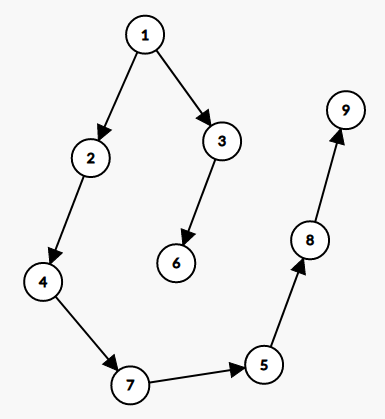
\includegraphics[width=0.8\linewidth]{Photos/HW1/dfs.png}
    \caption{درخت \lr{DFS} با شروع از راس ۱}
    \label{fig:my_label}
\end{figure}
با توجه به شکل فوق واضح است که از راس ۱ به همه‌ی رئوس مسیر وجود دارد. همچنین
اگر به درخت شکل فوق، یال‌های
\lr{(9, 1)}
و
\lr{(6, 8)}
از گراف اصلی را اضافه کنیم، دیده می‌شود که از هر راسی به راس ۱ نیز مسیر وجود دارد. در نتیجه بین هر راس دلخواه
\lr{u}
و
\lr{v}
نیز مسیر وجود دارد، زیرا می‌توان از
\lr{u}
به ۱ و همینطور از ۱ به
\lr{v}
رسید و بلعکس.

گراف
\lr{b}
قویا همبند نیست.\\
زیرا از راس ۶ به هیچ راسی مسیر نداریم ولی از بقیه رئوس به ۶ مسیر وجود دارد.

% --- Question 2 ---
% This section addresses the second question of the assignment.
\section*{سوال دوم}

% --- Part A: Adjacency Matrix ---
% This subsection provides the adjacency matrix for a given graph.
\subsection*{أ. ماتریس مجاورتی }

$\begin{pmatrix}
    0&1&1&0&0\\
    0&0&0&1&0\\
    0&1&0&0&1\\
    0&0&0&0&0\\
    0&0&0&1&0\\
\end{pmatrix}$

% --- Part B: Minimum Spanning Tree ---
% This subsection shows the Minimum Spanning Tree (MST) of a graph,
% found using Kruskal's algorithm.
\subsection*{ب. درخت کمینه‌ی پوشا}
با بکارگیری الگوریتم کروسکال، به ترتیب از کم‌ترین یال اضافه می‌کنیم تا شکل زیر بدست آید:
\begin{figure}[H]
    \center
    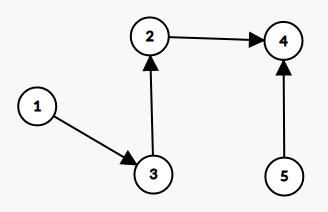
\includegraphics[width=0.8\linewidth]{Photos/HW1/mst.png}
    \caption{درخت کمینه‌ی پوشا}
    \label{fig:my_label}
\end{figure}

\end{multicols}
\end{document}
